%%%%%%%%%%%%%%%%%%%%%%%%%%%%%%%%%%%%%%%%%%%%%%%%%%%%%%%%%%%%%%%%%%%%%%%%%%%%%%%%%%
\begin{frame}[fragile]\frametitle{}

\begin{center}
{\Large Vector Representation of Words, aka Word Embeddings}

{\tiny (Ref:Introduction to Word Embeddings - Hunter Heidenreich )}

\end{center}

\end{frame}

%%%%%%%%%%%%%%%%%%%%%%%%%%%%%%%%%%%%%%%%%%%%%%%%%%%%%%%%%%%%%%%%%%%%%%%%%%%%%%%%%%
\begin{frame}[fragile]\frametitle{Why do we use word embeddings?}
  \begin{itemize}
    \item Computers can not process words
	\item They need numbers.
	\item Especially for Machine learning where we can apply mathematical rules and do matrix operations to them
  \end{itemize}


\end{frame}

%%%%%%%%%%%%%%%%%%%%%%%%%%%%%%%%%%%%%%%%%%%%%%%%%%%%%%%%%%%%%%%%%%%%%%%%%%%%%%%%%%
\begin{frame}[fragile]\frametitle{Why do we use word embeddings?}
  \begin{itemize}
    \item Another big advantage is that  is that we can actually pre-train word embeddings that are applicable to many tasks. 
	\item Only caution is that these embeddings are generic text corpus and carry general meanings.
	\item If you want domain specific meanings, then you will need to build your own word embeddings.
	\item ``Shell'' in zoology could mean creature houses you find on sea shore, but the same word in CAD means Hollowing operation.
	\item ``Draft'' in legal domain is a rough document, where as in CAD it is Tapering operation.
  \end{itemize}



\end{frame}


%%%%%%%%%%%%%%%%%%%%%%%%%%%%%%%%%%%%%%%%%%%%%%%%%%%%%%%%%%%%%%%%%%%%%%%%%%%%%%%%%%
\begin{frame}[fragile]\frametitle{What is a word embedding?}
  \begin{itemize}
    \item Word embedding = vector representation of a word
	\item A word is `embedded' in $n$ dimensional space.
	\item Once the words are vectors, their prosperities can be utilized.
	\item One such property is dot product giving cosine similarity.
	\item Goal is to capture some sort of relationship in that space, be it meaning, morphology, context, or some other kind of relationship.
  \end{itemize}


\end{frame}

%%%%%%%%%%%%%%%%%%%%%%%%%%%%%%%%%%%%%%%%%%%%%%%%%%%%%%%%%%%%%%%%%%%%%%%%%%%%%%%%%%
\begin{frame}[fragile]\frametitle{What is a word embedding?}
  \begin{itemize}
    \item The choice of $n$ in word embedding space, is our choice.
	\item It can be tens or hundreds instead of millions (like one-hot encoded vectors).
	\item A lot of word embeddings are created based on the notion introduced by Zellig Harris'``distributional hypothesis'' which boils down to a simple idea that words that are used close to one another typically have the same meaning.
	\item Different word embeddings are created either in different ways or using different text corpora to map this distributional relationship
  \end{itemize}


\end{frame}


%%%%%%%%%%%%%%%%%%%%%%%%%%%%%%%%%%%%%%%%%%%%%%%%%%%%%%%%%%%%%%%%%%%%%%%%%%%%%%%%%%
\begin{frame}[fragile]\frametitle{}

\begin{center}
{\Large Examples of Word Embeddings}

{\tiny (Ref:Introduction to Word Embeddings - Hunter Heidenreich )}

\end{center}

\end{frame}

%%%%%%%%%%%%%%%%%%%%%%%%%%%%%%%%%%%%%%%%%%%%%%%%%%%%%%%%%%%%%%%%%%%%%%%%%%%%%%%%%%
\begin{frame}[fragile]\frametitle{One-hot Encoding}
  \begin{itemize}
    \item Also called as Count Vectorizing
	\item A vector that has as many dimensions as your corpora has unique words. 
	\item Each unique word has a unique dimension and will be represented by a 1 in that dimension with 0s everywhere else.
  \end{itemize}
  
\begin{center}
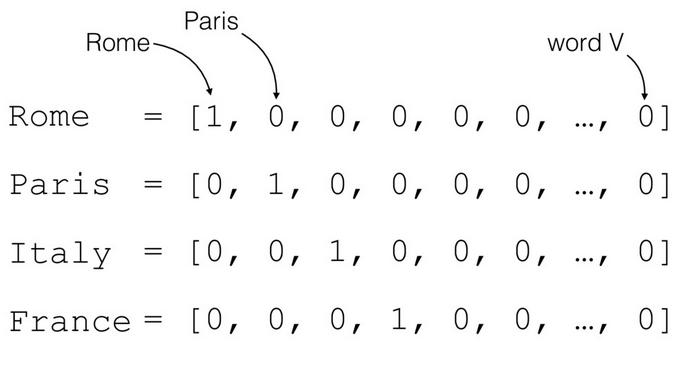
\includegraphics[width=0.6\linewidth,keepaspectratio]{w2v1}
\end{center}

Result: A really huge and sparse vectors that capture absolutely no relational information.
\end{frame}

%%%%%%%%%%%%%%%%%%%%%%%%%%%%%%%%%%%%%%%%%%%%%%%%%%%%%%%%%%%%%%%%%%%%%%%%%%%%%%%%%%
\begin{frame}[fragile]\frametitle{TF-IDF Transform}
  \begin{itemize}
    \item Related to one-hot encoded vectors
	\item Words are represented by their term frequency multiplied by their inverse document frequency.
	\item Words that occur a lot but everywhere should be given very little weighting or significance. 
	\item Words like ``the'' or ``and'' don't provide a large amount of value.
	\item  However, if a word appears very little or appears frequently, but only in one or two places, then its Imp and should be weighted High.
  \end{itemize}
  
\begin{center}
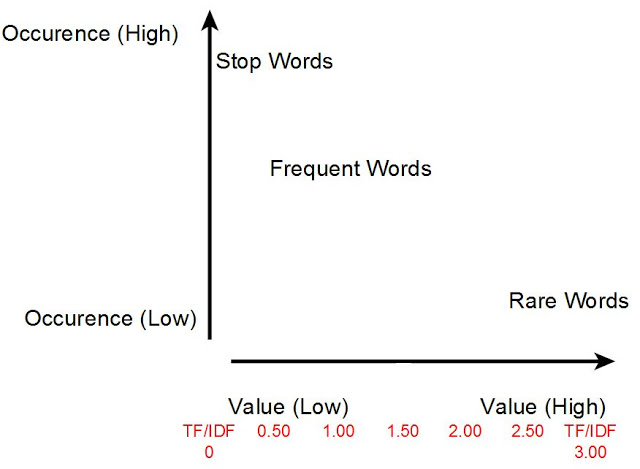
\includegraphics[width=0.4\linewidth,keepaspectratio]{w2v2}
\end{center}

This suffers from the downside of very high dimensional representations that don’t capture semantic relatedness.
\end{frame}

%%%%%%%%%%%%%%%%%%%%%%%%%%%%%%%%%%%%%%%%%%%%%%%%%%%%%%%%%%%%%%%%%%%%%%%%%%%%%%%%%%
\begin{frame}[fragile]\frametitle{Co-Occurrence Matrix}
  \begin{itemize}
    \item  A giant matrix that is as long and as wide as the vocabulary size. 
	\item If words occur together, they are marked with a positive entry. Otherwise, they have a 0. 
	\item Shows: ``Do words occur together? If yes, then count this.''
  \end{itemize}
  
\begin{center}
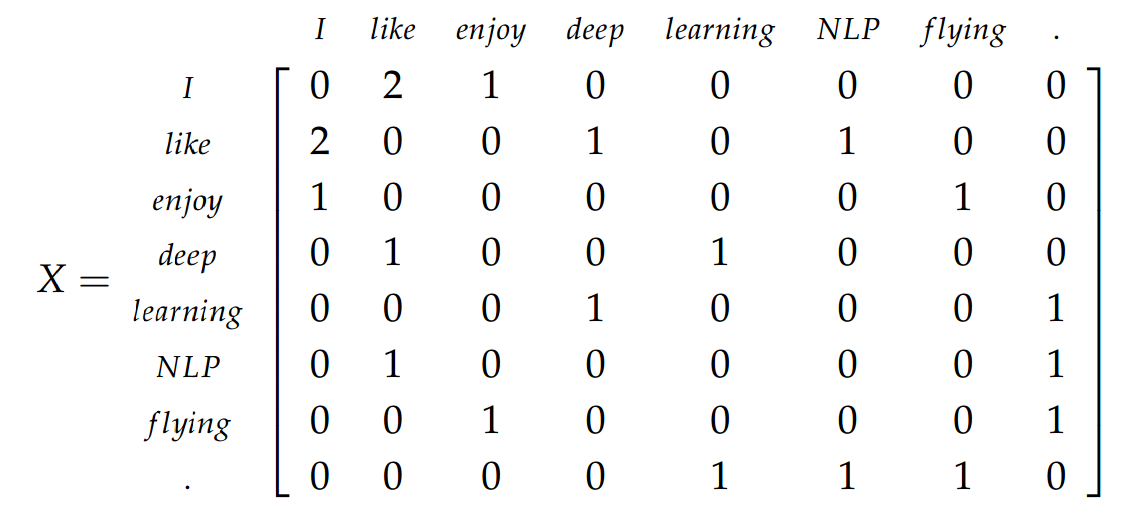
\includegraphics[width=0.6\linewidth,keepaspectratio]{w2v3}
\end{center}

If we thought that one-hot encoding was high dimensional, then co-occurrence is high dimensional squared.
\end{frame}



%%%%%%%%%%%%%%%%%%%%%%%%%%%%%%%%%%%%%%%%%%%%%%%%%%%%%%%%%%%%%%%%%%%%%%%%%%%%%%%%%%
\begin{frame}[fragile]\frametitle{Were these Good Vector Representations?}
\begin{itemize}
\item To have ''Semantic'' (meaning-wise) representation, the Similar words should be close to each other in the hyper dimensional space.
\item Non-similar words should be far apart from each other in the hyper dimensional space.
\end{itemize}
\end{frame}

%%%%%%%%%%%%%%%%%%%%%%%%%%%%%%%%%%%%%%%%%%%%%%%%%%%%%%%%%%%%%%%%%%%%%%%%%%%%%%%%%%
\begin{frame}[fragile]\frametitle{Were these Good Vector Representations?}
\begin{itemize}
\item Traditional One Hot Encoding:
	\begin{itemize}
	\item Apple = [1, 0, 0]
	\item Orange = [0, 1, 0]
	\item Plane = [0, 0, 1]
	\end{itemize}
\begin{center}
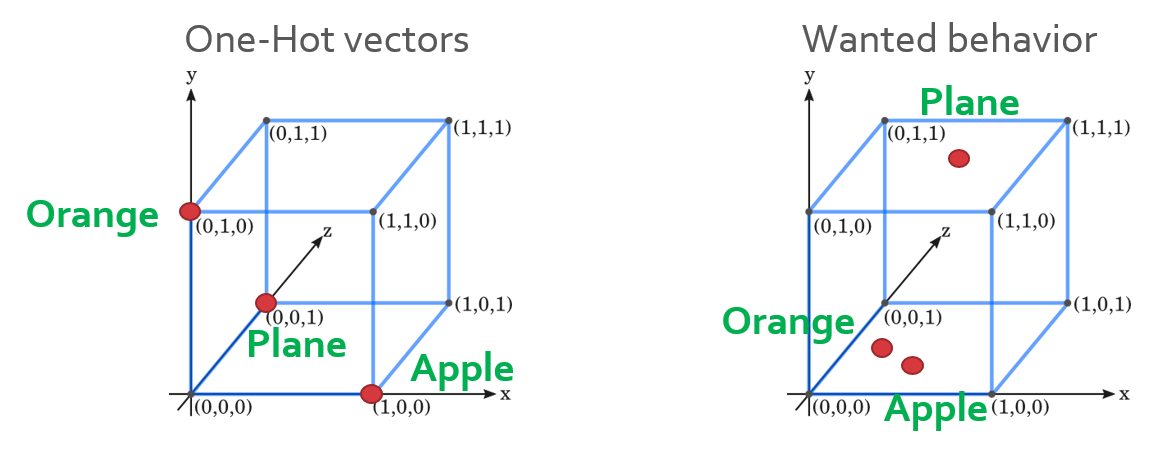
\includegraphics[width=0.8\linewidth,keepaspectratio]{word23_1}
\end{center}
\item Very few cells participate in the representation.
\end{itemize}
\end{frame}

%%%%%%%%%%%%%%%%%%%%%%%%%%%%%%%%%%%%%%%%%%%%%%%%%%%%%%%%%%%%%%%%%%%%%%%%%%%%%%%%%%
\begin{frame}[fragile]\frametitle{Neural Probabilistic Model}
  \begin{itemize}
    \item Learns an embedding by achieving some task like predicting context words, or center word etc
	\item Based on different neural network architectures.
	\item Typically, you clean your text and create one-hot encoded vectors. Then, you define your representation size (300 dimensional might be good). 
	\item It’s the entry point into the network, and back-propagation is utilized to modify the embedding based on whatever goal task we have.
  \end{itemize}
  
\end{frame}

%%%%%%%%%%%%%%%%%%%%%%%%%%%%%%%%%%%%%%%%%%%%%%%%%%%%%%%%%%%%%%%%%%%%%%%%%%%%%%%%%%
\begin{frame}[fragile]\frametitle{The Power of Word2Vecs}

\begin{itemize}
\item They provide a fresh perspective to ALL  problems in NLP, and not just solve one problem.
\item Technological Improvement
\item Rise of deep learning since 2006 (Big Data + GPUs  + Work done by Andrew Ng, Yoshua Bengio, Yann Lecun and Geoff Hinton)
\item Application of Deep Learning to NLP - led by Yoshua Bengio,  Christopher Manning, Richard Socher, Tomas Mikalov
\item The need for unsupervised learning. (Supervised learning tends to be excessively dependent on hand-labeled data and often does not scale)
\end{itemize}
\end{frame}


%%%%%%%%%%%%%%%%%%%%%%%%%%%%%%%%%%%%%%%%%%%%%%%%%%%%%%%%%%%%%%%%%%%%%%%%%%%%%%%%%%
\begin{frame}[fragile]\frametitle{Word Distributed Representation - Word2Vec}
\begin{itemize}
\item All vector cells participate in representing each word.
\item Words are represented by real valued dense vectors of significantly smaller dimensions (e.g. 100 - 1000).
\item  Intuition: consider each vector cell as a representative of some feature.
\begin{center}
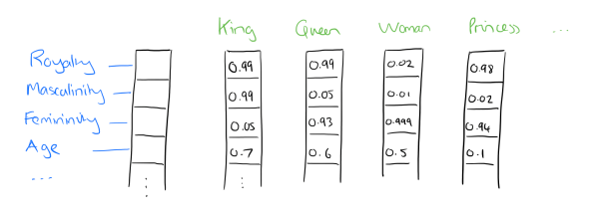
\includegraphics[width=\linewidth,keepaspectratio]{word24}
\end{center}
\end{itemize}
\end{frame}

%%%%%%%%%%%%%%%%%%%%%%%%%%%%%%%%%%%%%%%%%%%%%%%%%%%%%%%%%%%%%%%%%%%%%%%%%%%%%%%%%%
\begin{frame}[fragile]\frametitle{Examples}
Vectors for King, Man, Queen, \& Woman:
\begin{center}
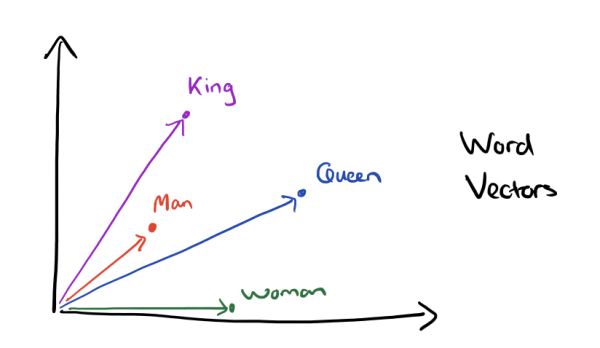
\includegraphics[width=0.5\linewidth,keepaspectratio]{word42}
\end{center}


\begin{center}
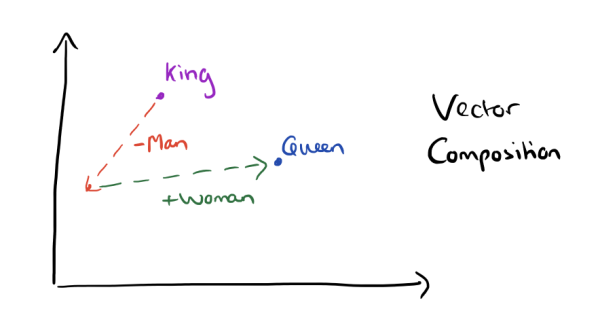
\includegraphics[width=0.5\linewidth,keepaspectratio]{word44}
\end{center}

\end{frame}

%%%%%%%%%%%%%%%%%%%%%%%%%%%%%%%%%%%%%%%%%%%%%%%%%%%%%%%%%%%%%%%%%%%%%%%%%%%%%%%%%%
\begin{frame}[fragile]\frametitle{Examples}
Gender relation:
\begin{center}
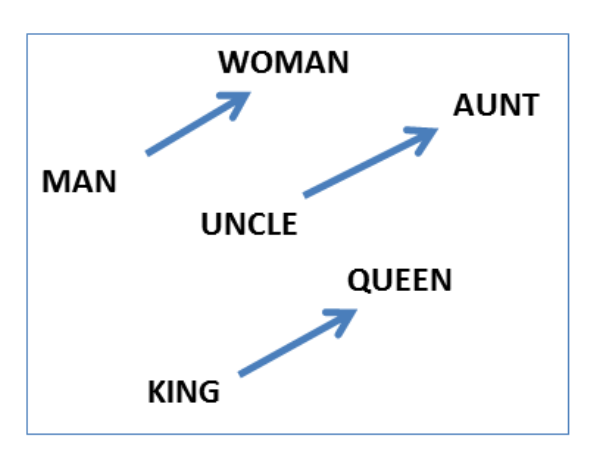
\includegraphics[width=0.4\linewidth,keepaspectratio]{word45}
\end{center}
Plural relation:

\begin{center}
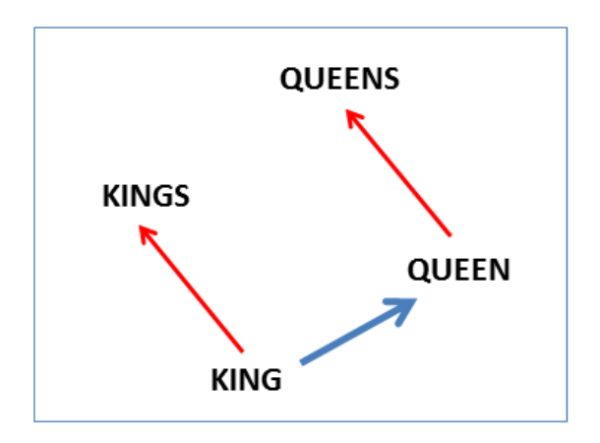
\includegraphics[width=0.4\linewidth,keepaspectratio]{word46}
\end{center}

\end{frame}

%%%%%%%%%%%%%%%%%%%%%%%%%%%%%%%%%%%%%%%%%%%%%%%%%%%%%%%%%%%%%%%%%%%%%%%%%%%%%%%%%%
\begin{frame}[fragile]\frametitle{Examples}
Word pair relationships:
\begin{center}
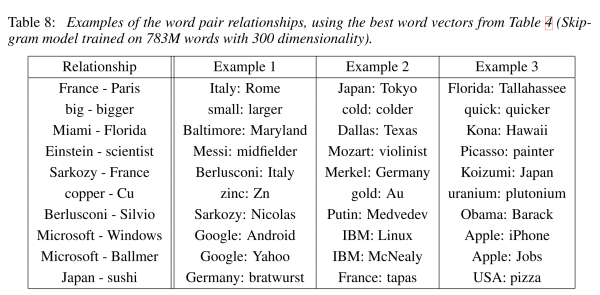
\includegraphics[width=0.8\linewidth,keepaspectratio]{word47}
\end{center}
\end{frame}

%%%%%%%%%%%%%%%%%%%%%%%%%%%%%%%%%%%%%%%%%%%%%%%%%%%%%%%%%%%%%%%%%%%%%%%%%%%%%%%%%%
\begin{frame}[fragile]\frametitle{Examples}
Country-capital city relationship:

\begin{center}
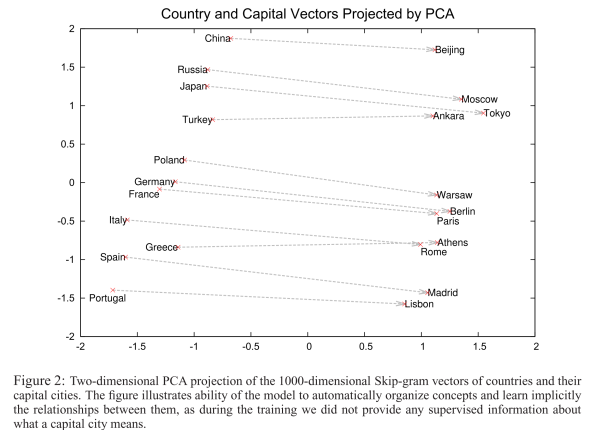
\includegraphics[width=0.8\linewidth,keepaspectratio]{word48}
\end{center}

\end{frame}



%%%%%%%%%%%%%%%%%%%%%%%%%%%%%%%%%%%%%%%%%%%%%%%%%%%%%%%%%%%%%%%%%%%%%%%%%%%%%%%%%%
\begin{frame}[fragile]\frametitle{Word2Vec}
Word2vec  (Google): a distributed representation of a word is used and not sparse like One-Hot.
\begin{center}
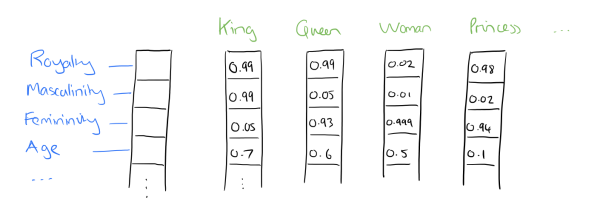
\includegraphics[width=0.8\linewidth,keepaspectratio]{word41}
\end{center}
Represent in some abstract way the `meaning' of a word.

\end{frame}


%%%%%%%%%%%%%%%%%%%%%%%%%%%%%%%%%%%%%%%%%%%%%%%%%%%%%%%%%%%%%%%%%%%%%%%%%%%%%%%%%%
\begin{frame}[fragile]\frametitle{Word2Vec}
Two major learning approaches:
  \begin{itemize}
    \item Continuous Bag-of-Words (CBOW): Learns an embedding by predicting the current words based on the context. The context is determined by the surrounding words.
	\item Continuous Skip-Gram: Learns an embedding by predicting the surrounding words given the context. The context is the current word.
  \end{itemize}
  
\begin{center}
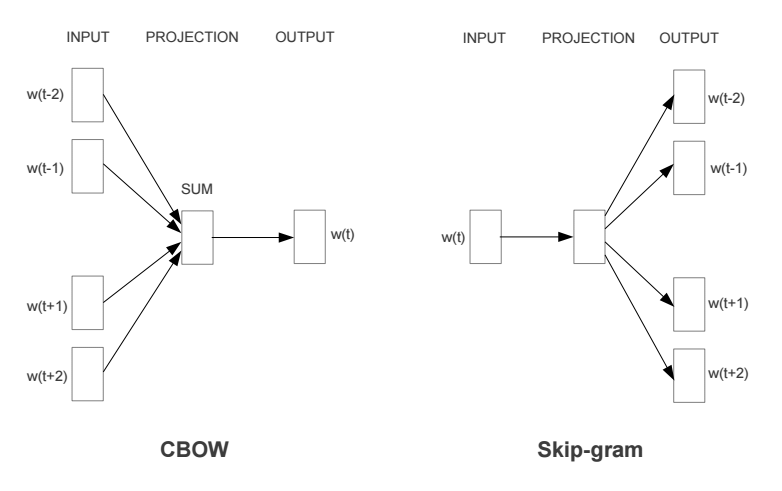
\includegraphics[width=0.7\linewidth,keepaspectratio]{w2v4}
\end{center}

\end{frame}

%%%%%%%%%%%%%%%%%%%%%%%%%%%%%%%%%%%%%%%%%%%%%%%%%%%%%%%%%%%%%%%%%%%%%%%%%%%%%%%%%%
\begin{frame}[fragile]\frametitle{Word2Vec}
  \begin{itemize}
    \item Both of these learning methods use local word usage context (with a defined window of neighboring words). 
	\item The larger the window is, the more topical similarities that are learned by the embedding. Forcing a smaller window results in more semantic, syntactic, and functional similarities to be learned.
  \end{itemize}

\end{frame}

%%%%%%%%%%%%%%%%%%%%%%%%%%%%%%%%%%%%%%%%%%%%%%%%%%%%%%%%%%%%%%%%%%%%%%%%%%%%%%%%%%
\begin{frame}[fragile]\frametitle{Benefits}
  \begin{itemize}
    \item Low space and low time complexity to generate a rich representation
	\item The larger the dimensionality, the more features we can have in our representation
	\item Allows us to efficiently generate something like a billion word corpora, 
	\item But encompass a bunch of generalities and keep the dimensionality small.
  \end{itemize}

\end{frame}

%%%%%%%%%%%%%%%%%%%%%%%%%%%%%%%%%%%%%%%%%%%%%%%%%%%%%%%%%%%%%%%%%%%%%%%%%%%%%%%%%%
\begin{frame}[fragile]\frametitle{Glove}
  \begin{itemize}
    \item An extension of word2vec, and a much better one at that.
	\item Contribution was the addition of global statistics in the language modeling task to generate the embedding. 
	\item There is no window feature for local context. 
	\item Instead, there is a word-context/word co-occurrence matrix that learns statistics across the entire corpora.
  \end{itemize}
  
\begin{center}
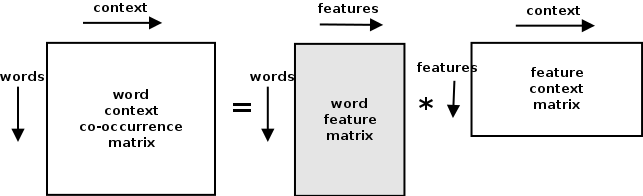
\includegraphics[width=0.7\linewidth,keepaspectratio]{w2v5}
\end{center}
  
\end{frame}

%%%%%%%%%%%%%%%%%%%%%%%%%%%%%%%%%%%%%%%%%%%%%%%%%%%%%%%%%%%%%%%%%%%%%%%%%%%%%%%%%%
\begin{frame}[fragile]\frametitle{FastText}
  \begin{itemize}
    \item To incorporate sub-word information by splitting all words into a bag of n-gram characters (typically of size 3-6). 
	\item It would add these sub-words together to create a whole word as a final feature. 
	\item Power: support out-of-vocabulary words! 
	\item n other approaches, if the system encounters a word that it doesn’t recognize, it just has to set it to the unknown word. With FastText, we can give meaning to words like circumnavigate if we only know the word navigate, because our semantic knowledge of the word navigate can help use at least provide a bit more semantic information to circumnavigate, even if it is not a word our system learned during training.
  \end{itemize}
  
 
\end{frame}

%%%%%%%%%%%%%%%%%%%%%%%%%%%%%%%%%%%%%%%%%%%%%%%%%%%%%%%%%%%%%%%%%%%%%%%%%%%%%%%%%%
\begin{frame}[fragile]\frametitle{FastText}
  \begin{itemize}
    \item Uses the skip-gram objective with negative sampling. 
	\item All sub-words are positive examples, and then random samples from a dictionary of words in the corpora are used as negative examples.
	\item Facebook, in developing FastText, has published pre-trained FastText vectors in 294 different languages.
  \end{itemize}
  
 
\end{frame}

%%%%%%%%%%%%%%%%%%%%%%%%%%%%%%%%%%%%%%%%%%%%%%%%%%%%%%%%%%%%%%%%%%%%%%%%%%%%%%%%%%
\begin{frame}[fragile]\frametitle{Poincare Embeddings (Hierarchal Representations)}
  \begin{itemize}
    \item Use hyperbolic geometry to capture hierarchal properties of words. 
	\item Hyperbolic space distance to encode similarity and the norm of vectors to encode hierarchal relationships.
	\item  Less dimensions are needed
  \end{itemize}
  
 \begin{center}
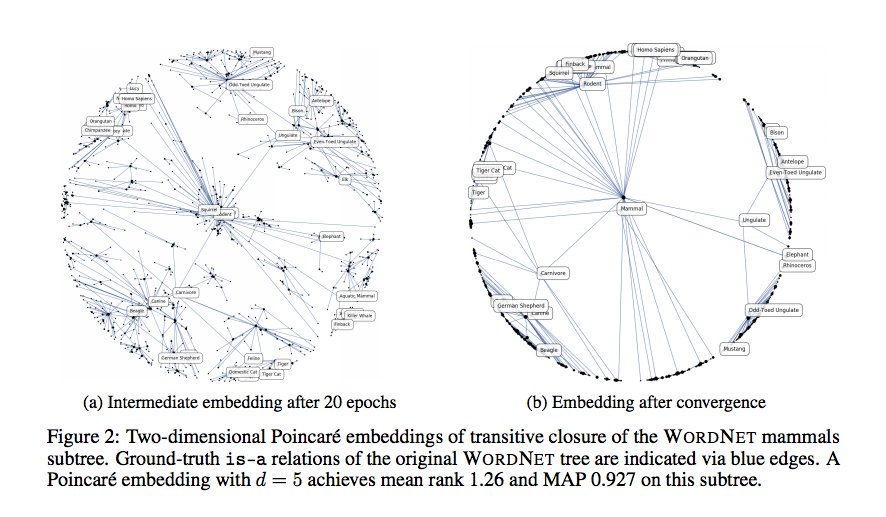
\includegraphics[width=0.6\linewidth,keepaspectratio]{w2v6}
\end{center}
\end{frame}

%%%%%%%%%%%%%%%%%%%%%%%%%%%%%%%%%%%%%%%%%%%%%%%%%%%%%%%%%%%%%%%%%%%%%%%%%%%%%%%%%%
\begin{frame}[fragile]\frametitle{ELMo}
  \begin{itemize}
    \item Generated from a function of the entire sentence to create word-level representations.
	\item The embeddings are generated at a character-level, so they can capitalize on sub-word units like FastText and do not suffer from the issue of out-of-vocabulary words.
	\item Trained as a bi-directional, two layer LSTM language model
	\item Lowest layer is good for things like POS tagging and other more syntactic and functional tasks, whereas the higher layer is good for things like word-sense disambiguation and other higher-level, more abstract tasks.
  \end{itemize}

\end{frame}


%%%%%%%%%%%%%%%%%%%%%%%%%%%%%%%%%%%%%%%%%%%%%%%%%%%%%%%%%%%%%%%%%%%%%%%%%%%%%%%%%%
\begin{frame}[fragile]\frametitle{Word Representations Comparison}

\adjustbox{valign=t}{
\begin{minipage}{0.45\linewidth}
Traditional Method  - Bag of Words Model

\begin{itemize}
\item Uses one hot encoding
\item Each word in the vocabulary is represented by one bit position in a HUGE vector.
\item For example, with a vocabulary of 10000 words, and ''Hello'' is the 4th word in the dictionary:  \lstinline|0 0 0 1 0 0  . . . . . . . 0 0 0 0 |
\item Context information is not utilized
\end{itemize}
\end{minipage}
}
\hfill
\adjustbox{valign=t}{
\begin{minipage}{0.45\linewidth}
Modern - Word Vectors

\begin{itemize}
\item Stores each word in as a point in space, represented by a vector of fixed number of dimensions (generally 300)
\item Unsupervised, built just by reading huge corpus
\item For example, ''Hello'' might be represented as :  \lstinline| [0.4, -0.11, 0.55, 0.3 . . . 0.1, 0.02]|
\item Context information is utilized
\end{itemize}
\end{minipage}
}
\end{frame}